\documentclass[]{aiaa-tc}% insert '[draft]' option to show overfull boxes

\usepackage{aiaa_packages}

 \title{Low-Thrust Trajectory Design Near Asteroids Using Reachability Sets}

 \author{
  Shankar Kulumani\thanksibid{1}%
    \thanks{Doctoral Student, \href{mailto:skulumani@gwu.edu}{skulumani@gwu.edu}. Student AIAA Member.}
  \ and Taeyoung Lee\thanksibid{2}\thanks{Associate Professor, \href{mailto:tylee@gwu.edu}{tylee@gwu.edu}. AIAA Member}\\
  {\normalsize\itshape
   Mechanical and Aerospace Engineering, George Washington University, 800 22nd St NW, Washington DC }\\
   }

 % Data used by 'handcarry' option if invoked
 \AIAApapernumber{YEAR-NUMBER}
 \AIAAconference{Conference Name, Date, and Location}
 \AIAAcopyright{\AIAAcopyrightD{YEAR}}

\begin{document}

\maketitle

\begin{abstract}
Write an awesome abstract

Use the reachability set to compute transfers

extend work already done in three body problem to motion around asteroid

Numerical example for asteroid 4769 Castalia
\end{abstract}

\section*{Nomenclature}

\begin{tabbing}
  XXX \= \kill% this line sets tab stop and adds a newline
  $J$ \> Jacobian Matrix \\
  $f$ \> Residual value vector \\
  $x$ \> Variable value vector \\
  $F$ \> Force, \si{\newton} \\
  $m$ \> Mass, \si{\kilo\gram} \\
  $\Delta x$ \> Variable displacement vector \\
  $\alpha$ \> Acceleration, \si{\meter\per\second\squared} \\[5pt]
  \textit{Subscript}\\
  $i$ \> Variable number \\
\end{tabbing}

\section{Introduction}\label{sec:introduction}

% Motivation for missions/studying asteroids
Small solar system bodies, such as asteroids and comets, are of significant interest to the scientific community.
These small bodies offer great insight into the early formation of the solar system.
This insight offers additional detail into the formation of the Earth and also the probable formation of other planetary systems.
Of particular interest are those near-Earth asteroids (NEA) which inhabit heliocentric orbits in vicinity of the Earth.
These easily accessible bodies provide attractive targets to support space industrialization, mining operations, and scientific missions..
NEAs potentially contain many materials useful for propulsion, construction, semiconductors, precious and strategic metals~\cite{ross2001}.
In addition, these NEAs are also of concern for their potential to impact the Earth~\cite{wie2008}.
Asteroids and comets are the greatest threat to future civilizations and as a result there is a focused effort to mitigate these risks.
In spite of the great interest in asteroids, the operation of spacecraft in thier vicinity is a challenging problem.

% Difficulty in system model
While there has been significant study of interplanetary transfer trajectories, relatively less analysis has been conducted on operations in the vicinity of asteroids.
The dynamic environment of around asteroids is strongly perturbed and challenging for analysis and mission operation.
Due to their small size and therefore low gravitational attraction asteroids have irregular shapes and potentially chaotic spin states.
Furthermore, due to the low gravitational attraction, other non-gravitional effects, such as solar radiation pressure, become more significant.
The orbital enviornment is in general quite complex and analytical insights are difficult to generate.

% Must estimate gravity and shape from ground based optical measurements
% most use a spherical harmonic model or a ellipsoid model but we use a polyhedron model
An accurate gravitional potential model is neccessary for the operation of spacecraft about asteroids.
Additionally, a detailed shape model of the asteroid is needed for trajectories passing close to the body.
The classic approach is to expand the gravitational potential into a harmonic series and compute the series coefficients.
Radio tracking data of an orbiting spacecraft allows one to estimate the series coefficients.
The harmonic representation are guaranteed to converge outside of the circumscribing sphere and can be truncated at a finite order based on accuracy requirements.
However, the harmonic expansion is always an approximation as a result of the infinite order series used in the representation.
Additionally, the harmonic model used outside of the circumscribing sphere is not guaranteed to converge inside the sphere.
As a result, additional steps must be taken to determine a valid harmonic expansion for particles close to the body.
This results in a cumbersome gravity field model that requires additional constraints to ensure continuity and validity at the radius of the circumscribing sphere~\cite{werner1996}.
Instead, we model the asteroid as a constant-density polyhedron and avoid the issues of the harmonic expansion while enabling several other useful advantages.

% benefits of the polyhedron model
A polyhedral model of the surface of an asteroid can be determined from remote optical or radar sensors.
The faces of the polyhedron can be large or small and allows for fine detail such as depression, craters, ridges, or interior voids.
In addition, there is no requirement for the body to be modeled at a uniformly high resolution so small details can be incorprated with minimal cost.
From the shape model, an analytical, closed form expression for the gravitational potential can be derived.
The polyhedral approach provides an accurate gravitational model consistent with the resolution of the shape and the chosen discretization.
Furthermore, the polyhedron model is an exact solution up to the surface of the body.
Therefore, this model is ideal for missions traversing large region both close and far from the asteroid.

% similarity to the three body problem
The irregular shape of asteroids leads to a richer dynamics as compard to the familar Kepler's problem, which is based on a point mass assumption.
The motion of particles around asteroids is modeled using the restricted full two-body problem.
This model has many similarities with the restricted three body problem, and much of the theory developed there is also applicable.
There has been much work in characterizing the relative equilibria and periodic orbits in the three-body problem.
In addition, orbital transfers have been designed which exploit the invariant manifolds of the three-body problem for low-energy manuevers~\cite{mingotti2011,grebow2011}.
The similarity of the three-body problem to motion around astreroids allows for much of the same theory to be applied to the asteroid problem.
More recently, the invariant manifolds around asteroids have been proposed for orbital transfers and landing manuevers~\cite{mondelo2010,herrera2014}.

% use of low thrust propulsion

The application of optimal control methods for orbital trajectory design is nontrivial.
In order to implement any optimization method a sufficiently accurate ``initial guess'' is required.
Frequently, insight into the problem or intuition on the part of the designer is often required to determine initial conditions that will converge to the optimal solution.
However, the asteroid system dynamics are nonlinear and exhibit chaotic behaviors.
This makes solving the optimization problem highly dependent on the initial condition.
Similar to the three-body problem, there is an insufficient number of analytical constants to derive an analytical solution in general.
As a result, accurate numerical methods are required to determine optimal solutions.
These methods are critically dependent on accurate initial guess in order to allow for convergence to an optimal solution.

% SYSTEMATIC DESIGN TO AVOID DIFFICULTIES IN CHOOSING A GOOD INITIAL GUESS
% CAPTURE LONG TERM EFFECTS OF LOW THRUST ACCURATELY IN NUMERICAL SIMULATION
In this paper, we extend the design method developed in the three-body problem to motion about asteroids~\cite{kulumani2015}.
Our approach avoids the difficulties in selecting an appropriate initial guess for optimization.
Instead, we utilize the concept of the reachability set to enable a simple methodology of selecting initial conditions to achieve general orbital transfers.
Given an initial condition and fixed time horizon, the reachable set is the set of states attainable, subject to the operational constraints of the spacecraft.
In addition, the generation of the reachable set allows for a more systematic method of determining initial conditions and eases the burden on the designer.
This simple methodology allows for extended transfer trajectories which iteratively approach a desired target orbit.


\section{Asteroid Model}\label{sec:asteroid_model}

\subsection{Shape Model}
Cite location of shape model database

Cite Scheeres orbits close to 4769 Castalia

Assuming constant rotation rate for asteroid

Mention we're looking at asteroid 4769 Castalia

\subsection{Polyhedron Gravity Model}\label{sec:polyhedron_model}

We represent the gravitational potential of the asteroid using a polyhedron gravitation model.
This model is composed of a polyhedron, a three-dimensional solid body, which is defined by a series of vectors in the body-fixed frame.
The vectors define vertices in the body-fixed frame as well as planar faces which compose the surface of the asteroid.
We assume that each face is a triangle composed of three vertices and three edges.
As a result, only two faces meet at each edge while three faces meet at each vertex.
Only the body-fixed vectors, and their associated topology, is required to define the exterior gravitational model.
References~\citenum{werner1994} and~\citenum{werner1997} give a detailed derivation of the polyhedron model.
Here, we summarize the key developments and equations required for implementation and clarity.

{\LARGE Insert picture of face and vectors}

Consider three vectors \( \vecbf{v}_1, \vecbf{v}_2, \vecbf{v}_3 \), assumed to be ordered in a counterclockwise direction, which define a face.
It is easy to define the three edges of each face as
\begin{align}\label{eq:edges}
    \vecbf{e}_{i+1,i} = \vecbf{v}_{i+1} - \vecbf{v}_i ,
\end{align}
where the index \( i \in \parenth{1,2,3} \) is used to permute all edges of each face.
Since each edge is a member of two faces, there exist two edges which are defined in opposite directions between the same vertices.
We can also define the outward normal vector to face \( f\)  as
\begin{align}\label{eq:face_normal}
    \hat{\vecbf{n}}_f &= \parenth{\vecbf{v}_{2} - \vecbf{v}_1} \times \parenth{\vecbf{v}_{3} - \vecbf{v}_2} ,
\end{align}
and the outward facing normal vector to each edge as
\begin{align}\label{eq:edge_normal}
    \hat{\vecbf{n}}_{i+1,i}^f &= \parenth{\vecbf{v}_{i+1} - \vecbf{v}_i} \times \hat{\vecbf{n}}_f .
\end{align}
For each face we define the face dyad \( \vecbf{F}_f \) as
\begin{align}\label{eq:face_dyad}
    \vecbf{F}_f &= \hat{\vecbf{n}}_f \hat{\vecbf{n}}_f .
\end{align}
Each edge is a member of two faces and has an outward pointing edge normal vector, given in~\cref{eq:edge_normal}, perpindicular to both the edge and the face normal.
For the edge connecting the vectors \( \vecbf{v}_1 \) and \( \vecbf{v}_2 \) which are shared between the faces \(A\) and \( B\) the per edge dyad is given by
\begin{align}\label{eq:edge_dyad}
    \vecbf{E}_{12} = \hat{\vecbf{n}}_A \hat{\vecbf{n}}_{12}^A + \hat{\vecbf{n}}_B \hat{\vecbf{n}}_{21}^B .
\end{align}
The edge dyad \( \vecbf{E}_e \) is defined for each edge and a function of the two adjacent faces meeting at the edge.
The face dyad \( \vecbf{F}_f \) is defined for each face and is a function of the face normal vector.

Let \( \vecbf{r}_i \) be the vector from the spacecraft to the vertex \( \vecbf{v}_i \) and it's length is \( r_i = \norm{\vecbf{r}_i} \).
The per-edge factor \( L_e \), for the edge connecting vertices \( \vecbf{v}_i \) and \( \vecbf{v}_j \), with a constant length \( e_{ij} \) is
\begin{align}\label{eq:edge_factor}
    L_e &= \ln \frac{r_i + r_j + e_{ij}}{r_i + r_j - e_{ij}}.
\end{align}
For the face defined by the vertices \( \vecbf{v}_i, \vecbf{v}_j, \vecbf{v}_k \) the per-face factor \( \omega_f \) is
\begin{align}\label{eq:face_factor}
    \omega_f &= 2 \arctan \frac{\vecbf{r}_i \cdot \vecbf{r}_j \times \vecbf{r}_k}{r_i r_j r_k + r_i \parenth{\vecbf{r}_j \cdot \vecbf{r}_k} + r_j \parenth{\vecbf{r}_k \cdot \vecbf{r}_i} + r_k \parenth{\vecbf{r}_i \cdot \vecbf{r}_j}} .
\end{align}
The gravitational potential due to a constant density polyhedron is given as
\begin{align}\label{eq:potential}
    U(\vecbf{r}) &= 1\frac{1}{2} G \sigma \sum_{e \in \text{edges}} \vecbf{r}_e \cdot \vecbf{E}_e \cdot \vecbf{r}_e \cdot L_e - \frac{1}{2}G \sigma \sum_{f \in \text{faces}} \vecbf{r}_f \cdot \vecbf{F}_f \cdot \vecbf{r}_f \cdot \omega_f
\end{align}
where \( \vecbf{r}_e, \vecbf{r}_f \) is the vector from the spacecraft to any point on the respective edge or face, \( G\) is the universal gravitational constant, and \( \sigma \) is the constant density of the asteroid.
Furthermore we can use these definitions to define the attraction, gravity gradient matrix, and Laplacian are defined as
\begin{align}
    \nabla U ( \vecbf{r} ) &= -G \sigma \sum_{e \in \text{edges}} \vecbf{E}_e \cdot \vecbf{r}_e \cdot L_e + G \sigma \sum_{f \in \text{faces}} \vecbf{F}_f \cdot \vecbf{r}_f \cdot \omega_f , \label{eq:attraction}\\
    \nabla \nabla U ( \vecbf{r} ) &= G \sigma \sum_{e \in \text{edges}} \vecbf{E}_e  \cdot L_e - G \sigma \sum_{f \in \text{faces}} \vecbf{F}_f \cdot \omega_f , \label{eq:gradient_matrix}\\
    \nabla^2 U &= -G \sigma \sum_{f \in \text{faces}}  \omega_f \label{eq:laplacian}.
\end{align}

One interesting thing to note is that both~\cref{eq:face_dyad,eq:edge_dyad} can be precomputed without knowledge of the position of the satellite.
They are both solely functions of the vertices and edges of the polyhedral shape model and are computed once and stored.
Once a position vector \( \vecbf{r} \) is defined then the scalars given in~\cref{eq:edge_factor,eq:face_factor} can be computed for each face and edge.
Finally,~\cref{eq:potential} is used to compute the gravitational potential on the spacecraft.

In this work, we consider trajectories about asteroid 4769 Castalia.
The shape model uses Doppler radar images to Castalia obstained at the Arecibo Observatory in 1989~\cite{hudson1994,neese2004}.
We use the estimated rotation period of \SI{4.07}{\hour} with a nominal density of \SI{2.1}{\gram\per\centi\meter\cubed}~\cite{scheeres1996}.
The shape model is composed of \num{4092} triangular faces and a rendering of the asteroid is provided in~\cref{fig:castalia_3d}.
In addition, we also show a contour plot of the radius of Castlia in~\cref{fig:radius_contour}.
\begin{figure}
    \centering
    \begin{subfigure}[htbp]{0.5\textwidth}
        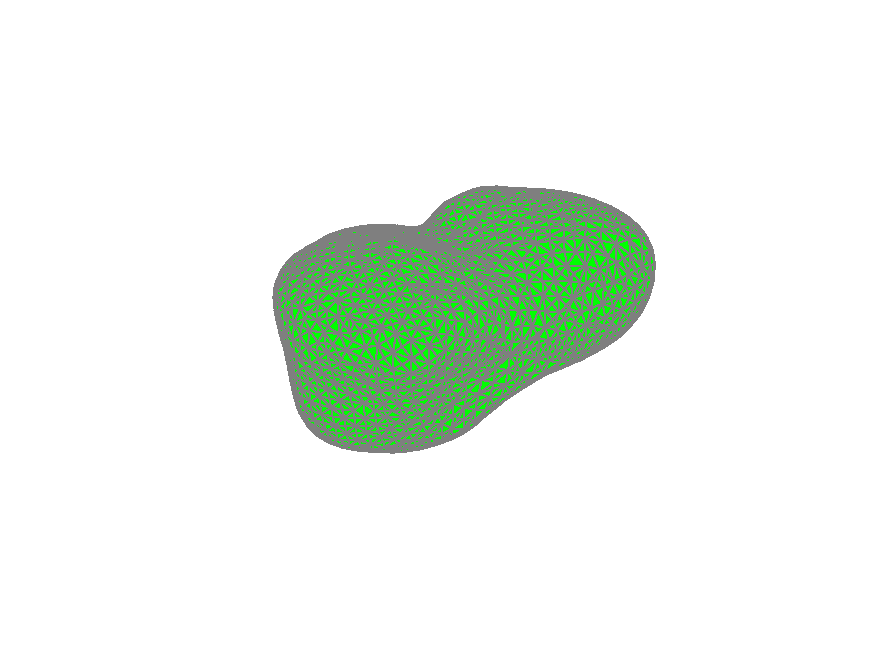
\includegraphics[width=\textwidth]{castalia}
        \caption{3D Shape Model of Castalia} \label{fig:castalia_3d}
    \end{subfigure}~ %add desired spacing between images, e. g. ~, \quad, \qquad, \hfill etc. %(or a blank line to force the subfigure onto a new line)
    \begin{subfigure}[htbp]{0.5\textwidth}
        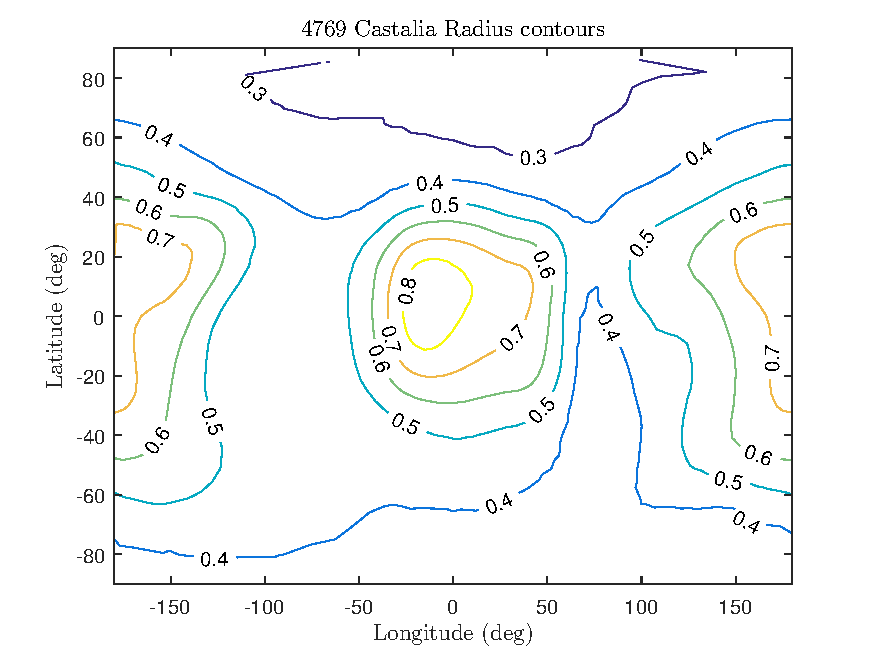
\includegraphics[width=\textwidth]{radius_contour}
        \caption{Radius contours of Castalia} \label{fig:radius_contour}
    \end{subfigure} ~ %add desired spacing between images, e. g. ~, \quad, \qquad, \hfill etc. %(or a blank line to force the subfigure onto a new line)
    \caption{Polyhedron Shape Model of 4769 Castalia}
    \label{fig:castalia}
\end{figure}


Mention that our model uses only 1024 faces for speed

Show the plot of the equilibrium position as a function of the number of faces and show that it's where the knee in the curve exists

\subsection{Spacecraft Equations of Motion}\label{sec:sc_eoms}

The motion of a massless particle, or spacecraft, about an asteroid shares many similarities with that of the three-body problem.
As is typical in the three-body problem, the equations of motion are usually represented in a uniformly rotating frame aligned with the two primaries.
Similarily, the equations of motion about an asteroid are also defined in a body-fixed frame with uniform rotation.
In this reference frame, the gravitational potential field is time invariant and only a function of the position of the particle.
In addition, since the rotational rate of the asteroid is constant the equations of motion are time invariant.
Finally, the use of the rotating reference frame allows for much greater insight into the dynamic structure of the behavior around the asteroid.

We define a reference frame originating at the center of mass of the asteroid.
The body-fixed reference frame is composed of the unit vectors \( \hat{\vecbf{x}} , \hat{\vecbf{y}}, \hat{\vecbf{z}} \), which are aligned along the principal axes of smallest, intermediate, and largest moment of inertia, respectively.
The body-fixed equations of motion of a massless particle about an arbitrarily rotating asteroid are given by
\begin{align}\label{eq:body_eoms}
    \ddot{\vecbf{r}} + 2 \vecbf{\Omega} \times \dot{\vecbf{r}} + \vecbf{\Omega} \times \parenth{ \vecbf{\Omega} \times \vecbf{r} } + \dot{\vecbf{\Omega}} \times \vecbf{r} = U_{\vecbf{r}} ,
\end{align}
where \( \vecbf{\Omega} \) is the instaneous angular velocity vector of the asteroid represented in the body-fixed frame, \( \vecbf{r} \) is the position of the particle in the body-fixed frame, and \( U_{\vecbf{r}} \) is the gradient of the gravitational potential~\cite{scheeres2012a}.
We assume that the asteroid rotates at a uniform rate, \( \norm{\vecbf{\Omega}} = \omega \), about the axis of the maximum moment of inertia, \( \vecbf{\Omega} = \omega \hat{\vecbf{z} }\).
As a result, we can represent the equations of motion in scalar form as
\begin{align} \label{eq:eoms}
    \begin{split}
        \ddot{x} - 2 \omega \dot{y} - \omega^2 y &= U_x , \\
        \ddot{y} + 2 \omega \dot{x} - \omega^2 x &= U_y , \\
        \ddot{z} &= U_z .
    \end{split}
\end{align}

We assume that in our problem we are modelling a spacecraft rather than a massless particle.
In this situation, the state is defined as \( \vecbf{x} = \begin{bmatrix}\vecbf{r} &\vecbf{v} \end{bmatrix}^T\) with \(\vecbf{r} = \begin{bmatrix} x & y & z \end{bmatrix}^T \in \R^{3\times1}\) and \(\vecbf{v}= \begin{bmatrix} \dot{x} & \dot{y} & \dot{z} \end{bmatrix}^T \in \R^{3\times1}\) representing the position and velocity with respect to the body-fixed frame, respectively.
We further assume that our spacecraft is capable of exerting a translational force, \( \vecbf{u} \in \R^{3\times1} \), in any direction, while subject to a maximum magnitude constraint.
This is typical of many spacecraft which offer full rotational freedom and can direct a maximum, and potentially varying, thrust in any direction.
The equations of motion may be rewritten in state space form as
\begin{align}\label{eq:state_space_eoms}
    \begin{bmatrix} \dot{\vecbf{r}} \\ \dot{\vecbf{v}} \end{bmatrix} &=
    \begin{bmatrix}\vecbf{v} \\ \vecbf{g} \parenth{\vecbf{r}} + \vecbf{h}\parenth{\vecbf{v}} + \vecbf{u} \end{bmatrix} ,
\end{align}
where the terms \(\vecbf{g} \parenth{\vecbf{r}} \) and \( \vecbf{h}\parenth{\vecbf{v}} \) are given by
\begin{align}\label{eq:state_space_terms}
    \vecbf{g}\parenth{\vecbf{r}} = \begin{bmatrix}  U_x + \omega^2 x \\ U_y + \omega^2 y \\ U_z \end{bmatrix} ,\quad
    \vecbf{h}\parenth{\vecbf{r}} = \begin{bmatrix} 2 \omega \dot{y} \\ -2 \omega \dot{x} \\ 0 \end{bmatrix} .
\end{align}

Since Castalia is a uniformly rotating asteroid, the equations of motion are time invariant when represented in the body-fixed frame.
In addition, there exists an integral of motion, or a conserved quantity, the is constant for all motion of a particle, absent any other perturbing forces.
The Jacobi constant, \( J (\vecbf{r} , \vecbf{v} ) \), is given by
\begin{align}\label{eq:jacobi}
    J \parenth{\vecbf{r}, \vecbf{v}} = \frac{1}{2} \omega^2 \parenth{x^2 + y^2} + U(\vecbf{r}) - \frac{1}{2} \parenth{\dot{x}^2 + \dot{y}^2 + \dot{z}^2} .
\end{align}
The Jacobi constant functions in a similar manner as used in three-body problem~\cite{szebehely1967}.
We can define zero-velocity surfaces using the Jacobi constant by fixing the value to a desired constant.
The zero-velocity surfaces are the locus of points where the kinetic energy and hence velocity vanishes.
Just as in the three-body problem, the Jacobi constant in~\cref{eq:jacobi} divides the phase space into distinct realms of possible motion.
Similarly, there exist in general four equilibrium points and also their associated stable and unstable manifolds~\cite{scheeres1996,scheeres1994}.
The properties of these manifolds play a critical role in the dynamics of trajecotries in their vicinity.

\section{Reachability Set on \Poincare Section}\label{sec:reachability}

Typical optimal control methods, including both indirect and direct based methods, are highly dependent on an accurate initial guess.
For indirect optimization, which is based on the calclus of variations, this results in the well-known two-point boundary value problem.
Insight into the problem or insight by the designer is usually required to determine appropriate initial costates that will converge to the optimal solution and satisfy the desired constraints.
To avoid this issue, we utilize the concept of the reachiblity set on a lower dimensional \Poincare section.
By repeatedly constructing the reachability set we can achieve general transfers by determining set intersections on the \Poincare section.
This alleviates the need to determine an accurate initial guess while offering some insight into the dynamics of neighboring trajectories

The reachable set contains all possible trajectories that are achievable over a fixed time horizon from a defined initial condition, subject to the constraints of the system.
Reachability theory has been applied to collision avoidance and safety planning in aerospace systems~\cite{holzinger2009,holzinger2011b}.
The theory supporting reachabiilty analysis is directly derivable from optimal control theory~\cite{varaiya2000,lygeros2004}.
Analytic, computation of reachability sets is only possible for a small class of potential systems.
Here, we use numerical methods to solve an optimal control problem.
The solution of this optimal control problem approximates a single solution that lies on the reachable set.
\begin{figure}
    \centering
    \begin{scaletikzpicturetowidth}{0.5\textwidth}
    \begin{tikzpicture}[scale=\tikzscale]
        \coordinate [label=left:\textcolor{black}{\large \(\vec{x}_0\)}] (x0) at (-1,-2);
        \coordinate [label=below:\textcolor{black}{\large  \(\vec{x}_n\)}] (xn) at (1,1);
        \coordinate [label=left:\textcolor{black}{\large  \(\Sigma\)}] (sigma) at (-4,3);
        %\coordinate [label=below:\textcolor{black}{\large  \(P(\vec{x})\)}] (P) at (0,-3.5);
        % define the path of the flow with coordinates
        \coordinate [label=right:\textcolor{black}{}] (f1) at (5,-2);
        \coordinate [label=below:\textcolor{black}{\large  \(\phi(t,\vec{x}_0)\)}] (f2) at (2,-5);
        \coordinate [label=right:\textcolor{black}{}] (f3) at (-4,-4);
        \coordinate [label=right:\textcolor{black}{}] (f4) at (-4,-1);
        
    %   \draw[help lines] (-10,-10) grid (10,10); %grid
        \filldraw [black] (x0) circle [radius=3pt];
        \filldraw [black] (xn) circle [radius=3pt];
    
        \draw [ultra thick,black,->-](x0) to[out=20,in=90,distance=2cm] (f1) to[out=-90,in=0,distance=2cm] (f2) to[out=180,in=-45,distance=2cm] (f3) to[out=135,in=-135,distance=2cm] (f4) ;
        \draw [ultra thick, black,dashed,->] (f4) to[out=45,in=180,distance=1cm] ($(xn)-(2,0)$);
        
        \draw [ultra thick] plot [smooth cycle, tension=0.1, rotate=5] coordinates { (-4,-3) (4,-3) (4,3) (-4,3) };
    
        \draw [thick,dashed] (xn) circle [radius=2cm]; % reachability set
    
        \draw [thick,->] (xn) -- ($(xn) + (2.5,0)$);
        \draw [thick,rotate=45,->] (xn) -- ($(xn) + (2.5,0)$);
        \draw ($(xn) + (1,0)$) arc [start angle=0,end angle=45, radius=1];
        \node [draw=none] at (2.4,1.5) {\Large \(\theta_d\)};
        \draw [decorate,decoration={brace,amplitude=5pt},rotate=45] (xn) -- ($(xn) + (2,0)$);
        \node [draw=none] at ($ (xn) + (0,1) $) {\Large \( J \)};
    \end{tikzpicture}
    \end{scaletikzpicturetowidth}
    \caption{Reachability set on a \Poincare section\label{fig:reachability_set}}
\end{figure}

We seek to approximate the reachability set on a \Poincare section by solving an optimal control problem.
The \Poincare section is chosen in a manner similar to the previous work in both the three-body problem as well analysis performed around asteroids to determine periodic orbits.
Analysis in the three-body problem relies heaviliy on symmetries in the force fields.
However, in our system model the gravitational potential, given by~\cref{eq:potential}, has no symmetries.
In spite of this, it is still possible to determine periodic solutions through the application of a \Poincare map with surface of section chosen normal to surface in the phase space~\cite{scheeres2000}.
For a periodic orbit, the trajectories will intersect the \Poincare section at two distinct points every half orbit.
With the addition of a low thrust control input, we are able to expand the reachable set from a distinct point to a larger area on the \Poincare section.
\Cref{fig:reachability_set} illustrates this methodology.
Without any control input, the trajectories will intersect the \Poincare section at \( \vecbf{x}_n\).
The addition of a control input allows the spacecraft to depart from the natural dynamics and intersect the section at another location.
We use the cost function \( J \) to define a distance metric on the \Poincare section.
Maximization of \( J \), or the minimization of \( -J \), along various directions on the \Poincare section allows us to generate the larges reachability set under the bounded control input.

We define the \Poincare section as the surface normal to \( y = 0 \).
Following convention, the \Poincare map is defined as the map from one transversal crossing of the surface \( y = 0\) to the next.
Using the method of Reference~\cite{scheeres2000}, we are able to remove \( y \) and \( \dot{y} \), creating a four-dimensional map.
The \Poincare section, \( \Sigma \) then becomes
\begin{align}\label{eq:poincare_section}
    \Sigma = \braces{\parenth{x, \dot{x}, z, \dot{z}} | y(t_f) = 0 }.
\end{align}
We use this section to compute periodic orbits that serve as the initial and target of our transfer.
In addition, this section serves as a lower dimensional space upon which we approximate the reachability set.

An optimal control problem is defined by the cost function
\begin{align}\label{eq:cost}
    J = -\frac{1}{2} \left( \vecbf{x}(t_f) - \vecbf{x}_{n}(t_f)\right)^T 
    \begin{bmatrix}
        1 & 0 & 0 & 0 & 0 & 0 \\
        0 & 0 & 0 & 0 & 0 & 0 \\
        0 & 0 & 1 & 0 & 0 & 0 \\
        0 & 0 & 0 & 1 & 0 & 0 \\
        0 & 0 & 0 & 0 & 0 & 0 \\
        0 & 0 & 0 & 0 & 0 & 1 \\
    \end{bmatrix}
    \left( \vecbf{x}(t_f) - \vecbf{x}_{n}(t_f)\right) ,
\end{align}
where \( \vecbf{x}_n(t_f) \) is the final state of a control-free trajectory, while the term \( \vecbf{x}(t_f)\) is the final state of a trajectory under the influence of the control input.
Maximization of the distance between \( \vecbf{x}_n \) and \(\vecbf{x} \), on the \Poincare section defined in~\cref{eq:poincare_section}, is equivalent to the minimization of \( J \) defined in~\cref{eq:cost}.
We ensure that the trajectories intersect the \Poincare section through the use of terminal constraints.
In addition, we use the terminal constraints to define a specific direction along which we seek to minimize the cost~\cref{eq:cost}.
Since the \Poincare section is four-dimensional we parameterize a direction in \( \R^4 \)  using three angles \( \phi_1, \phi_2 , \phi_3 \) to define the terminal constraints
\begin{align}\label{eq:terminal_constraints}
    \begin{split}
        m_1 &= y = 0 \\
        m_2 &= \parenth{\sin \phi_{1_{d}}} \parenth{ x_1^2 + x_2^2 + x_3^2 + x_4^2} - x_1^2 = 0, \\
        m_3 &= \parenth{\sin \phi_{2_{d}}} \parenth{ x_2^2 + x_3^2 + x_4^2} - x_2^2 = 0, \\
        m_4 &= \parenth{\sin \phi_{3_{d}}} \parenth{ 2 x_3^2 + 2 x_3 \sqrt{x_4^2 + 2 x_4^2}} - x_3 - \sqrt{x_4^2 + x_3^2} = 0. 
    \end{split}
\end{align}
We make use of the difference states \( \parenth{x_1, x_2 ,x_3, x_4 }\) which are defined as
\begin{align}\label{eq:diff_states}
    \begin{split}
        x_1 &= x(t_f) - x_n(t_f) , \\
        x_2 &= z(t_f) - z_n(t_f) , \\
        x_3 &= \dot{x}(t_f) - \dot{x}_n(t_f) , \\
        x_4 &= \dot{z}(t_f) - \dot{z}_n(t_f) . \\
    \end{split}
\end{align}
The constraint \( m_1 = 0 \) ensures that the terminal states lies on the \Poincare section.
The constraints \( m_2, m_3, m_4 \) are used to define a direction on the \Poincare section.
Finally, we also incorporate a control thrust magnitude constraint given by
\begin{align}\label{eq:control_constraint}
    c(\vecbf{u}) = \vecbf{u}^T \vecbf{u} - u_m^2 \leq 0 ,
\end{align}
where \( u_m \) is the maximum thrust magnitude.
This constraint assumes that the control thrust may be orientated in any direction yet the thrust is variable but limited.
The goal is to determine the control history \( \vecbf{u}(t) \) such that teh cost function~\cref{eq:cost} is minimized while subject to the equations of motion~\cref{eq:body_eoms} and the constraints~\cref{eq:control_constraint,eq:terminal_constraints}.

% How do you solve the optimal control problem
We apply a standard calculus of variations approach to solve our optimal control problem~\cite{bryson2002}.
Using the Euler-Lagrange equations we arrive at the necessary conditions for optimality
\begin{align}\label{eq:necc_conditions}
    \begin{split}
        \dot{\vecbf{x}} ^T &= \deriv{H}{\vecbf{\lambda}} ,\\
        \dot{\vecbf{\lambda}}^T &= \deriv{H}{\vecbf{x}} , \\
        0 &= \deriv{\phi}{x}^T + \deriv{\vecbf{m}}{x}^T \vecbf{\beta} - \vecbf{\lambda}^T(t_f) , \\
        0 &= \deriv{H}{\vecbf{u}} + \mu^T \deriv{c}{\vecbf{u}} ,
    \end{split}
\end{align}
where the Hamiltonian, \( H\), is defined as
\begin{align}\label{eq:hamiltonian}
    H = \vecbf{\lambda}_r^T \vecbf{v} + \vecbf{\lambda}_v^T \parenth{\vecbf{g}(\vecbf{r}) + \vecbf{h}(\vecbf{v}) + \vecbf{u}}.
\end{align}
The costate is given by \( \vecbf{\lambda} = \begin{bmatrix} \vecbf{\lambda}_r & \vecbf{\lambda}_v \end{bmatrix}^T \in \R^{6 \times 1}\), \( \vecbf{\beta} \in \R^{4 \times 1} \) are the additional Lagrange multiplers associated with the terminal constraints in~\cref{eq:terminal_constraints}, and \( \mu \) is a Lagrange multipler associated with the control constraint in~\cref{eq:control_constraint}.

We can redefine the optimal control in terms of the costate by rewritting the necessary condition as
\begin{align*}
    \vecbf{u} = - \frac{u_m^2}{2 \mu} \vecbf{\lambda}_v .
\end{align*}
We use this along with the control constraint to solve for the Lagrange multipler \( \mu \)
\begin{align*}
    \mu = \pm \frac{u_m}{2} \norm{\vecbf{\lambda}_v} .
\end{align*}
Finally, we use the second-order necessary condition to determine the correct sign of \( \mu \) and find the optimal control input for the reachable set as
\begin{align}\label{eq:optimal_control}
    \vecbf{u} = - u_m \frac{\vecbf{\lambda}}{\norm{\vecbf{\lambda}}} .
\end{align}

This optimal control formulation results in a two point boundary value problem.
We use a shooting method to determine the initial costates, \( \vecbf{\lambda}(t_0)\), such that the terminal constraints are satisfied.
In addition, we implement a multiple shooting method which sub-divides the the entire trajectory into small sub-intervals~\cite{stoer2013}.
We incorporate additional interior constraints to ensure a continuous trajectory at the patch points between the sub-intervals.
The multiple shooting method reduces the sensitivity of the terminal states to the initial conditions and alleviates many of the issues of single shooting approaches.

\section{Numerical Simulation}\label{sec:simulation}

We present an example transfer of a spacecraft about the asteroid 4769 Castalia. 
Our equations of motion, given by~\cref{eq:eoms}, are an idealized version of the dynamics of a spacecraft.
For example, the model does not include the effect of mass transfer from propellant usage. 
We instead model the control input as a generic acceleration vector in the body-fixed asteroid frame. 
The thrust magnitude constraint in~\cref{eq:control_constraint} is chosen to emulate a physically realizable thruster system.
In this analysis, we assume \( u_m = \SI{0.1}{\milli\meter\per\second\squared}\) which is equivalent to a thrust of approximately \SI{100}{\milli\newton} for a \SI{1000}{\kilo\gram} spacecraft.
This amount of thrust is typical of many current ion or hall effect thrusters and is in operation in several current missions (cite Goebels Fundamentals of electric propulsion and Dawn thruster paper by choueiri2009new).

The objective is to transfer the spacecraft between two periodic equatorial orbits about Castalia.
The initial and target orbits are periodic solutions about Castlia computed using the method introduced by Reference~\citenum{scheeres2003}.
The initial conditions for both orbits are defined in the body-fixed frame as
\begin{align}\label{sec:initial_transfer}
    \vecbf{x}_i = 
    \begin{bmatrix}
        1.4973 \\ 0 \\ 0.0061 \\ 0\\ -0.0009 \\ 0
    \end{bmatrix} ,
    \quad
    \vecbf{x}_t =
    \begin{bmatrix}
        2.9786 \\ 0 \\ 0.0012 \\ 0\\ -0.0011 \\ 0
    \end{bmatrix} .
\end{align}
\Cref{fig:initial_transfer} shows the initial and desired periodic orbits which lie in the equatorial plane of Castalia.
Our goal is to transfer from a lower altitude to a higher altitude while remaining in the equatorial plane of the asteroid.
This type of scenario would occur frequently during mapping and observation missions to asteroids.
\begin{figure}[htbp]
    \centering 
    \begin{subfigure}[htbp]{0.5\textwidth} 
        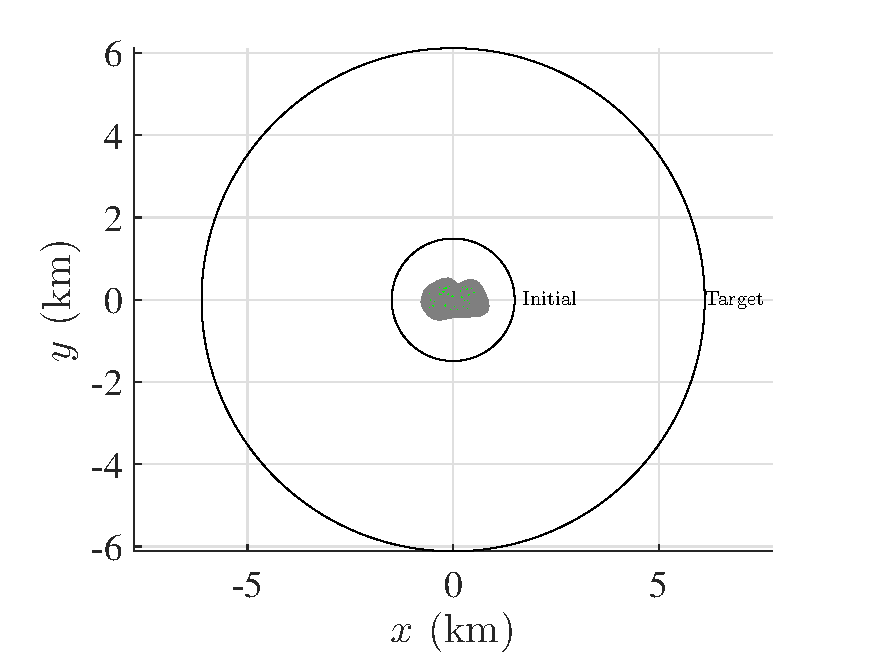
\includegraphics[width=\textwidth]{initial_transfer} 
        \caption{Equatorial View} \label{fig:eq_initial_transfer} 
    \end{subfigure}~ %add desired spacing between images, e. g. ~, \quad, \qquad, \hfill etc. %(or a blank line to force the subfigure onto a new line) 
    \begin{subfigure}[htbp]{0.5\textwidth} 
        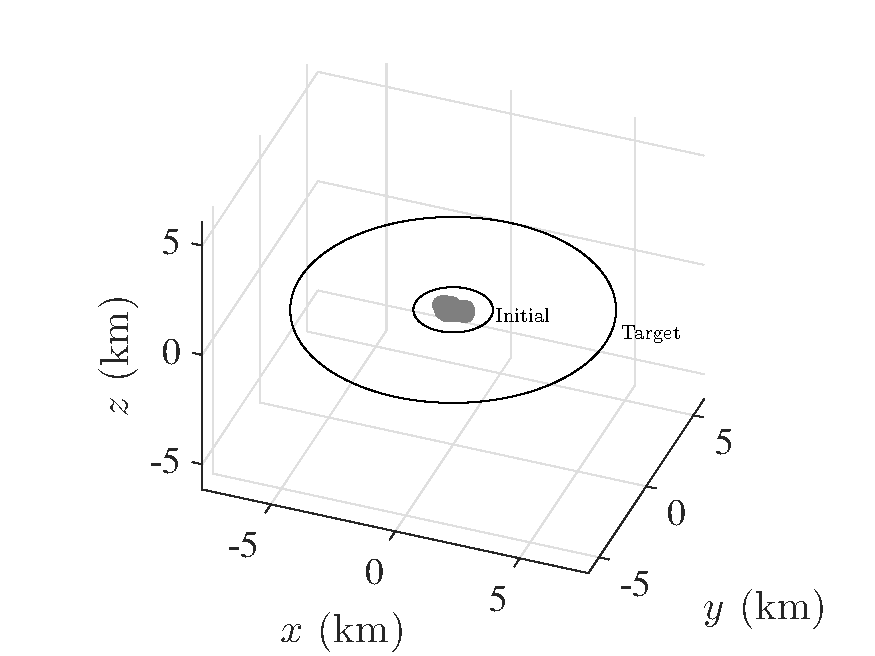
\includegraphics[width=\textwidth]{initial_transfer_3d} 
        \caption{3D view} \label{fig:initial_transfer_3d} 
    \end{subfigure} ~ %add desired spacing between images, e. g. ~, \quad, \qquad, \hfill etc. %(or a blank line to force the subfigure onto a new line) 
    \caption{Initial and target periodic orbits}
    \label{fig:initial_transfer} 
\end{figure}
In this transfer example we also have used a reduced model of Castalia.
Rather than using the full \num{4092} face model we reduce the number of faces to \num{1024}. 
This greatly speeds up the computation with only a small difference in the potential field or shape model.

We first compute the reachability set originating from the initial periodic orbit at \( \vecbf{x}_i\) for a fixed time of flight and bounded control magnitude as defined preivously.
Since the target periodic orbit also lies in the equatorial plane, we augment~\cref{eq:terminal_constraints} with an additional constraint \( m_5 = z = 0\) to ensure that the trajectories remain in the equatorial plane.
The reachability set is computed by solving the two-point boundary value problem using a multiple shooting algorithm to satisfy the necessary conditions in~\cref{eq:necc_conditions}.
The reachability set is generated on the lower dimensional \Poincare section and is composed of the terminal states in the \( \parenth{x,z,\dot{x},\dot{z} } \) space.
We visualize the section using the two figures in~\cref{fig:poincare_section}.
\begin{figure}[htbp]
    \centering 
    \begin{subfigure}[htbp]{0.5\textwidth} 
        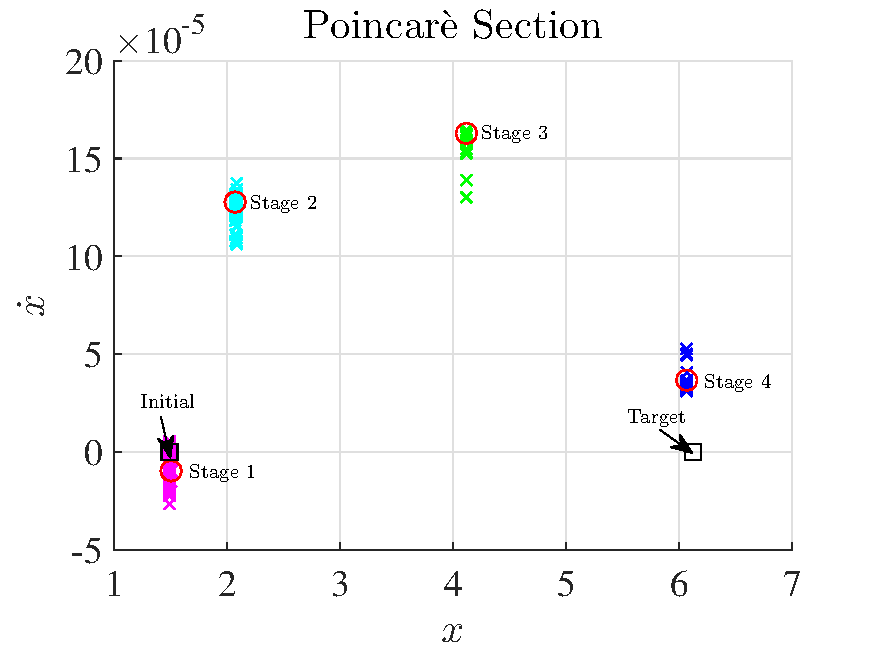
\includegraphics[width=\textwidth]{figures/poincare_xvsxdot.pdf} 
        \caption{\( x \) vs. \( \dot{x} \) \Poincare section} \label{fig:poincare_xvsxdot} 
    \end{subfigure}~ %add desired spacing between images, e. g. ~, \quad, \qquad, \hfill etc. %(or a blank line to force the subfigure onto a new line) 
    \begin{subfigure}[htbp]{0.5\textwidth} 
        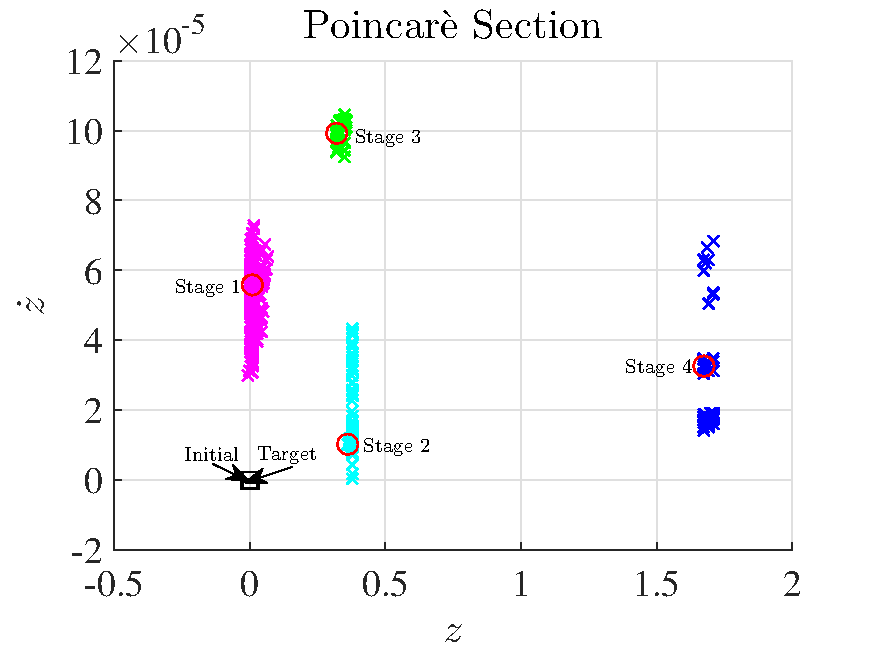
\includegraphics[width=\textwidth]{figures/poincare_zvszdot.pdf} 
        \caption{\( z \) vs. \( \dot{z} \) \Poincare section} \label{fig:poincare_zvszdot} 
    \end{subfigure}
    \caption{\Poincare section visualization}
    \label{fig:poincare_section} 
\end{figure}
These two-dimensional sections allow us to visualize the four-dimensional \Poincare section of~\cref{eq:poincare_section}.


we use a lower number of faces to speed up the computation

Transfer is between equatorial periodic orbits in the body fixed frame

We compute the reachability set given a fixed initial state over a fixed time span

We then determine the state(which is on the reachability set) which minimizes the distance to the target

This state is used to intialize the next stage

Repeat this until we can achieve both position coordinates on the various \Poincare sections

The velocities do not match but a simple optimal control scheme is used to arrive at the target

Transfer about asteroid Castalia - cite some Scheeres papers

Plots of \Poincare section

Full trajectory plots


\section{Conclusions}\label{sec:conclusions}


\section*{Acknowledgments}\label{sec:aknowledgments}

A place to recognize others.

\bibliographystyle{aiaa}
\bibliography{library}

\end{document}
